\chapter{Assessment of Government Intervention}\label{ch:assessment}

\section{Economic Rationale}\label{sec:rationale}

Each instrument is assessed by the constraint it addresses, the incentives it creates, and the distribution of its costs and benefits. Correlated losses justify public risk-sharing, and the costs of information and delivery justify attention to insurance infrastructure \citep{miranda1997,mahul2010}. Affordability and redistribution can justify premium assistance, but they do not determine a particular rate \citep{hazell2017}. Production can respond to changes in price, access, or risk-bearing under any of the three instruments, so the rollout comparisons in Chapter~\ref{ch:results} test a possible consequence of insurance availability as a package, not the effect of any single instrument.

\section{Premium Subsidies}\label{sec:premium}

Let $P$ be the pure premium per unit of coverage and $s$ the combined national and local subsidy rate, so that the policyholder price is $(1 - s)P$. With coverage demand $D(\cdot)$, coverage purchased without and with support is
\begin{equation}\label{eq:demand}
q_{0} = D(P),\qquad q_{1} = D\bigl((1 - s)P\bigr).
\end{equation}

Figure~\ref{fig:premiumsupport} assumes perfectly elastic supply at $P$. The subsidy raises coverage from $q_{0}$ to $q_{1}$ at a public cost of $sPq_{1}$, of which $sPq_{0}$ is a transfer to purchases that would have occurred without support.

\begin{figure}[htbp]
\centering
\IfFileExists{"insurance graph.tex"}{%
  \adjustbox{max width=\textwidth}{\input{"insurance graph"}}%
}{%
  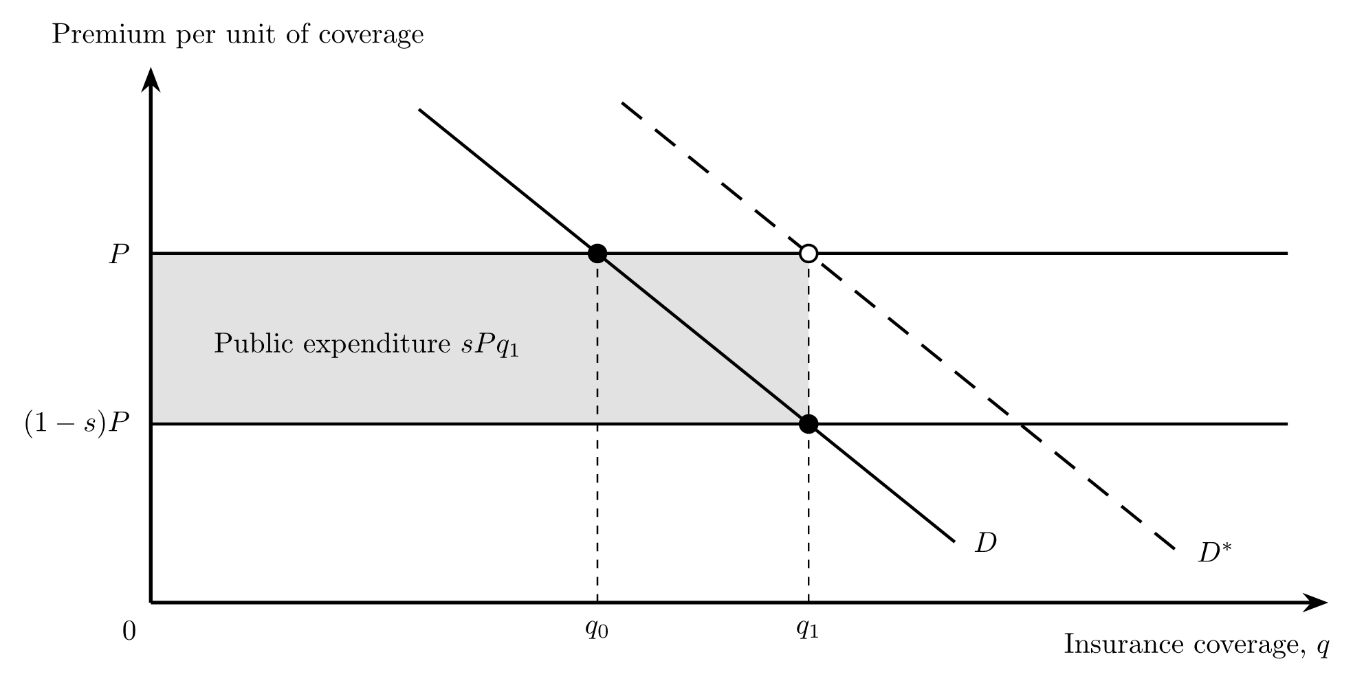
\includegraphics[width=\textwidth]{figures/fig4_premium_support_fallback.png}%
}
\caption{Premium Support and the Demand for Insurance Coverage}\label{fig:premiumsupport}
\notes{$P$ is the pure premium per unit of coverage and $s$ the combined subsidy rate. Supply is perfectly elastic at $P$, and the loading is financed separately. $D$ is observed demand; $D^{*}$ is demand when the value of protection is fully perceived. The shaded rectangle is public pure-premium support, $sPq_{1}$, a transfer rather than a welfare loss. Arbitrary units.}
\end{figure}

Figure~\ref{fig:premiumsupport} is a partial-equilibrium illustration for a given risk class with a fixed premium and loading financed separately. Its shaded rectangle measures a public transfer. If willingness to pay captures protection benefits and $P$ equals marginal resource cost, coverage beyond $q_{0}$ creates an allocative loss. If demand understates those benefits, $D^{*}$ illustrates a possible rationale for additional coverage. Differences in risk preferences, liquidity, and information need not produce the same demand shift, and changes in the insured risk pool can alter premiums. The diagram therefore explains possible mechanisms rather than identifying an optimal subsidy rate or measuring Korean welfare gains.

The 2026 national schedule supports 33-65 percent of the pure premium for specified product-coverage combinations and 50 percent for others, subject to a national subsidy ceiling of KRW 50 million per policyholder per product \citep[p.~2]{mafra2026}. At a fixed subsidy rate, support rises with the eligible premium until this ceiling binds; beyond it, additional premiums receive no additional national subsidy. This limits large transfers but does not target household income. Local assistance must be considered separately. For products sold from July 2026, policyholders with a five-year cumulative loss ratio of at least 500 percent cannot select coverage of 80 percent or higher. Individual loss experience enters premium adjustments for products sold from November 2026 \citep{mafra2026}. Greater risk differentiation can strengthen pricing incentives while reducing affordable protection for repeatedly affected farms.

\section{Administrative Cost Subsidies}\label{sec:administrative}

The 2026 rules distinguish the risk premium and loss-investigation expenses, which together form the pure premium, from the loading, which includes delegated selling and other specified operating costs. Public support covers the loading in full \citep{mafra2026}. Loss-investigation costs should therefore be identified separately when comparing administrative expenditure, rather than counted again as part of the loading. The relevant economic question is whether financing delivers coverage and timely, accurate settlement at a reasonable resource cost.

Comparable indicators require consistent numerators and denominators. Selling and policy-servicing expenditure can be expressed per active contract, and claim-assessment expenditure per completed claim. Product and regional comparisons should also report the operating-cost-to-premium ratio, using a stated premium definition, alongside settlement duration and assessment corrections. Differences in risk prices, claim frequency, product complexity, and geographical dispersion can move these ratios without changing efficiency. Comparisons within similar product and risk categories are consequently more informative than an aggregate international ranking.

Mahul and Stutley \citeyearpar[pp.~84-87]{mahul2010} emphasize the role of low-cost delivery channels. A performance-linked component of administrative payments could reward timely settlement and verified assessment quality, while a separate component maintains access in costly areas. Rewarding closure speed alone could encourage premature or inaccurate settlement. These incentive trade-offs matter independently of whether the aggregate subsidy rises or falls.

\section{State Reinsurance}\label{sec:reinsurance}

State reinsurance provides capacity for correlated losses in exchange for a contingent public liability. A stop-loss contract with attachment point $a$ splits total covered claims $L$ into retained and ceded portions:
\begin{equation}\label{eq:stoploss}
L^{ret} = \min(L,a),\qquad L^{ced} = \max(L - a,0).
\end{equation}

Under a proportional contract, by contrast, the state receives a share of the premium and bears the same share of claims. Korea moved from a stop-loss contract with a 180 percent attachment point in 2005-2013 to a mixed stop-loss and profit-and-loss-sharing arrangement, introduced in 2014 and applied to the whole program from 2019 \citep[pp.~268, 273-274]{mafra2025}. Figure~\ref{fig:reinsurance} contrasts the two benchmark forms. The 50 percent first-stage state share used in Panel B does not fully represent the Korean contract.

In the uncapped stop-loss benchmark, private claims do not rise beyond the attachment point; actual incentives also depend on treaty limits, pricing, and renewal. Proportional sharing preserves marginal private exposure but transfers a share of ordinary losses to the state. The appropriate allocation depends on loss correlation and relative risk-bearing capacity \citep{jia2025}. With reinsurance premium $R$, expressed in the same units as $L$ and $a$, the expected public cost under stop-loss is expected ceded claims minus the premium received:
\begin{equation}\label{eq:publiccost}
E[C] = E\bigl[\max(L - a,0)\bigr] - R.
\end{equation}

Reported crop reinsurance payments over 2005-2024 total KRW 923.8 billion, against receipts of KRW 470.0 billion \citep[p.~269]{mafra2025}. The KRW 453.8 billion difference is a nominal cumulative cash-flow measure, not an inflation-adjusted cost series or the fund's complete financial balance. Actuarial adequacy instead compares premiums with expected losses and risk-bearing costs under each treaty. Comparisons over time must distinguish changes in prices, insured exposure, coverage, contract terms, and settlement dates. Dividing payments by insured hectares alone would not adjust for differences in insured value or loss severity.

\begin{figure}[htbp]
\centering
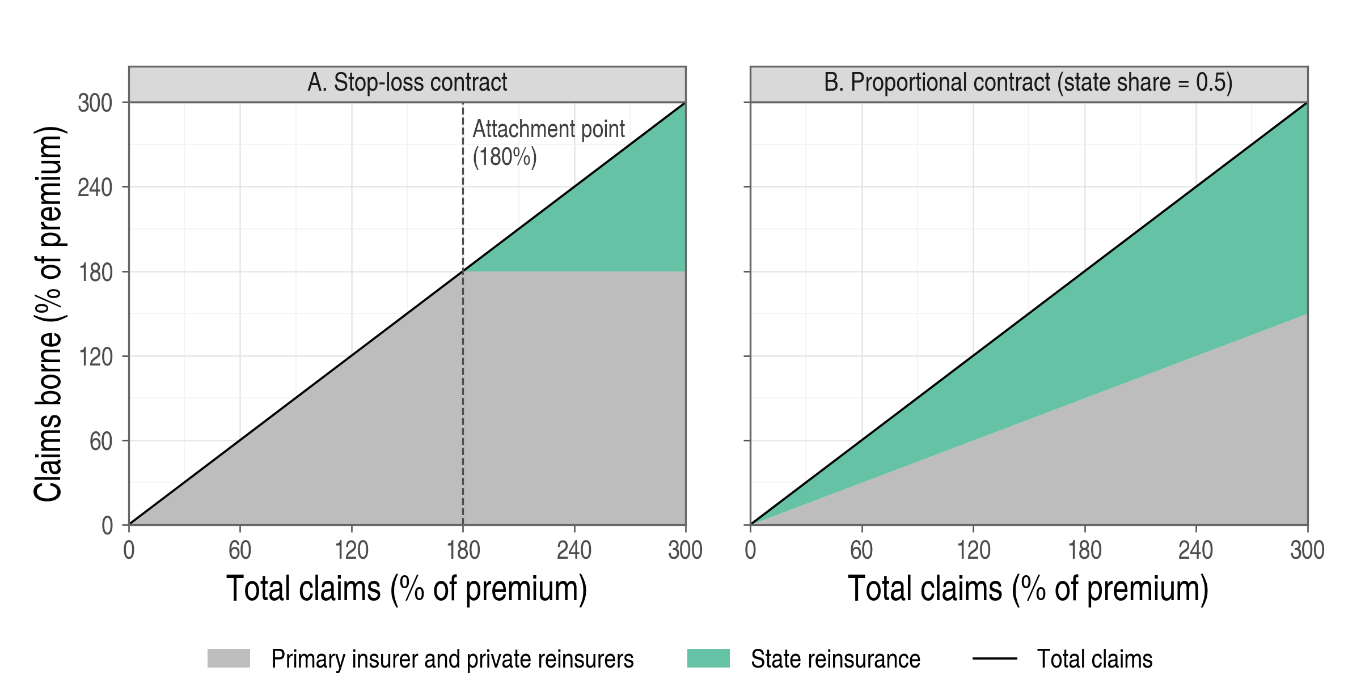
\includegraphics[width=\textwidth]{figures/fig5_reinsurance_allocation.png}
\caption{Allocation of Claims under Stop-Loss and Proportional Reinsurance}\label{fig:reinsurance}
\notes{Both axes express claims as percentages of premium. Panel A uses the 180 percent attachment point reported for 2005-2013 \citep[p.~273]{mafra2025}. Private claims combine those of the operator and private reinsurers. In both panels, the private and state shares are stacked and sum to total claims. Panel B is an illustrative proportional contract without additional layers, premium transfers, expenses, or commissions.}
\end{figure}

A forward-looking assessment should distinguish expected net cost, liquidity when claims fall due, and exposure to severe or consecutive loss years. Each requires the treaty schedule, premiums, reserves, and committed financing. Catastrophe exposure depends on loss dependence as well as frequency and severity \citep{mahul2010,kang2017}. Historical payments should be evaluated under the contracts in force at the time rather than retrospectively applying current sharing rates.
